%\chapter{Gestión del plan de estudios}
% [JGC]: esto es copy/paste de lo que se había iniciado hace dos años
\chapter{Gestión curricular}
En este apartado se plantea componentes necesarios para la administración educativa de la malla curricular, incluyendo el plan de transición para estudiantes activos del plan de estudios vigente. También se aborda la evaluación curricular posterior a su futura implementación y la forma en que el personal docente será capacitado a las nuevas exigencias de la malla curricular.

\section{Administración y ejecución}

\subsection{Estructura administrativa de la unidad académica}

La carrera Bachillerato y Licenciatura en Matemática pertenece al Departamento de Matemática y Ciencias Actuariales, el cual actualmente administra también la carrera Bach. y Lic. en Ciencias Actuariales. En la Figura \ref{fig:dpto} se presenta la estructura administrativa vigente. Con la creación del Departamento de Ciencias Actuariales, el Departamento de Matemática está a cargo exclusivamente de la carrera de Matemática y la administración de cursos de matemática de la carrera de Ciencias Actuariales. Esto permitirá un enfoque especializado en temas de plan de estudios, investigación, acción social y apoyo a estudiantes, buscando potenciar ambas carreras a nivel nacional e internacional. Además, en eventuales procesos de autoevaluación y acreditación, cada departamento podrá concentrar esfuerzos en cada carrera específica.

\begin{figure}
    \centering
    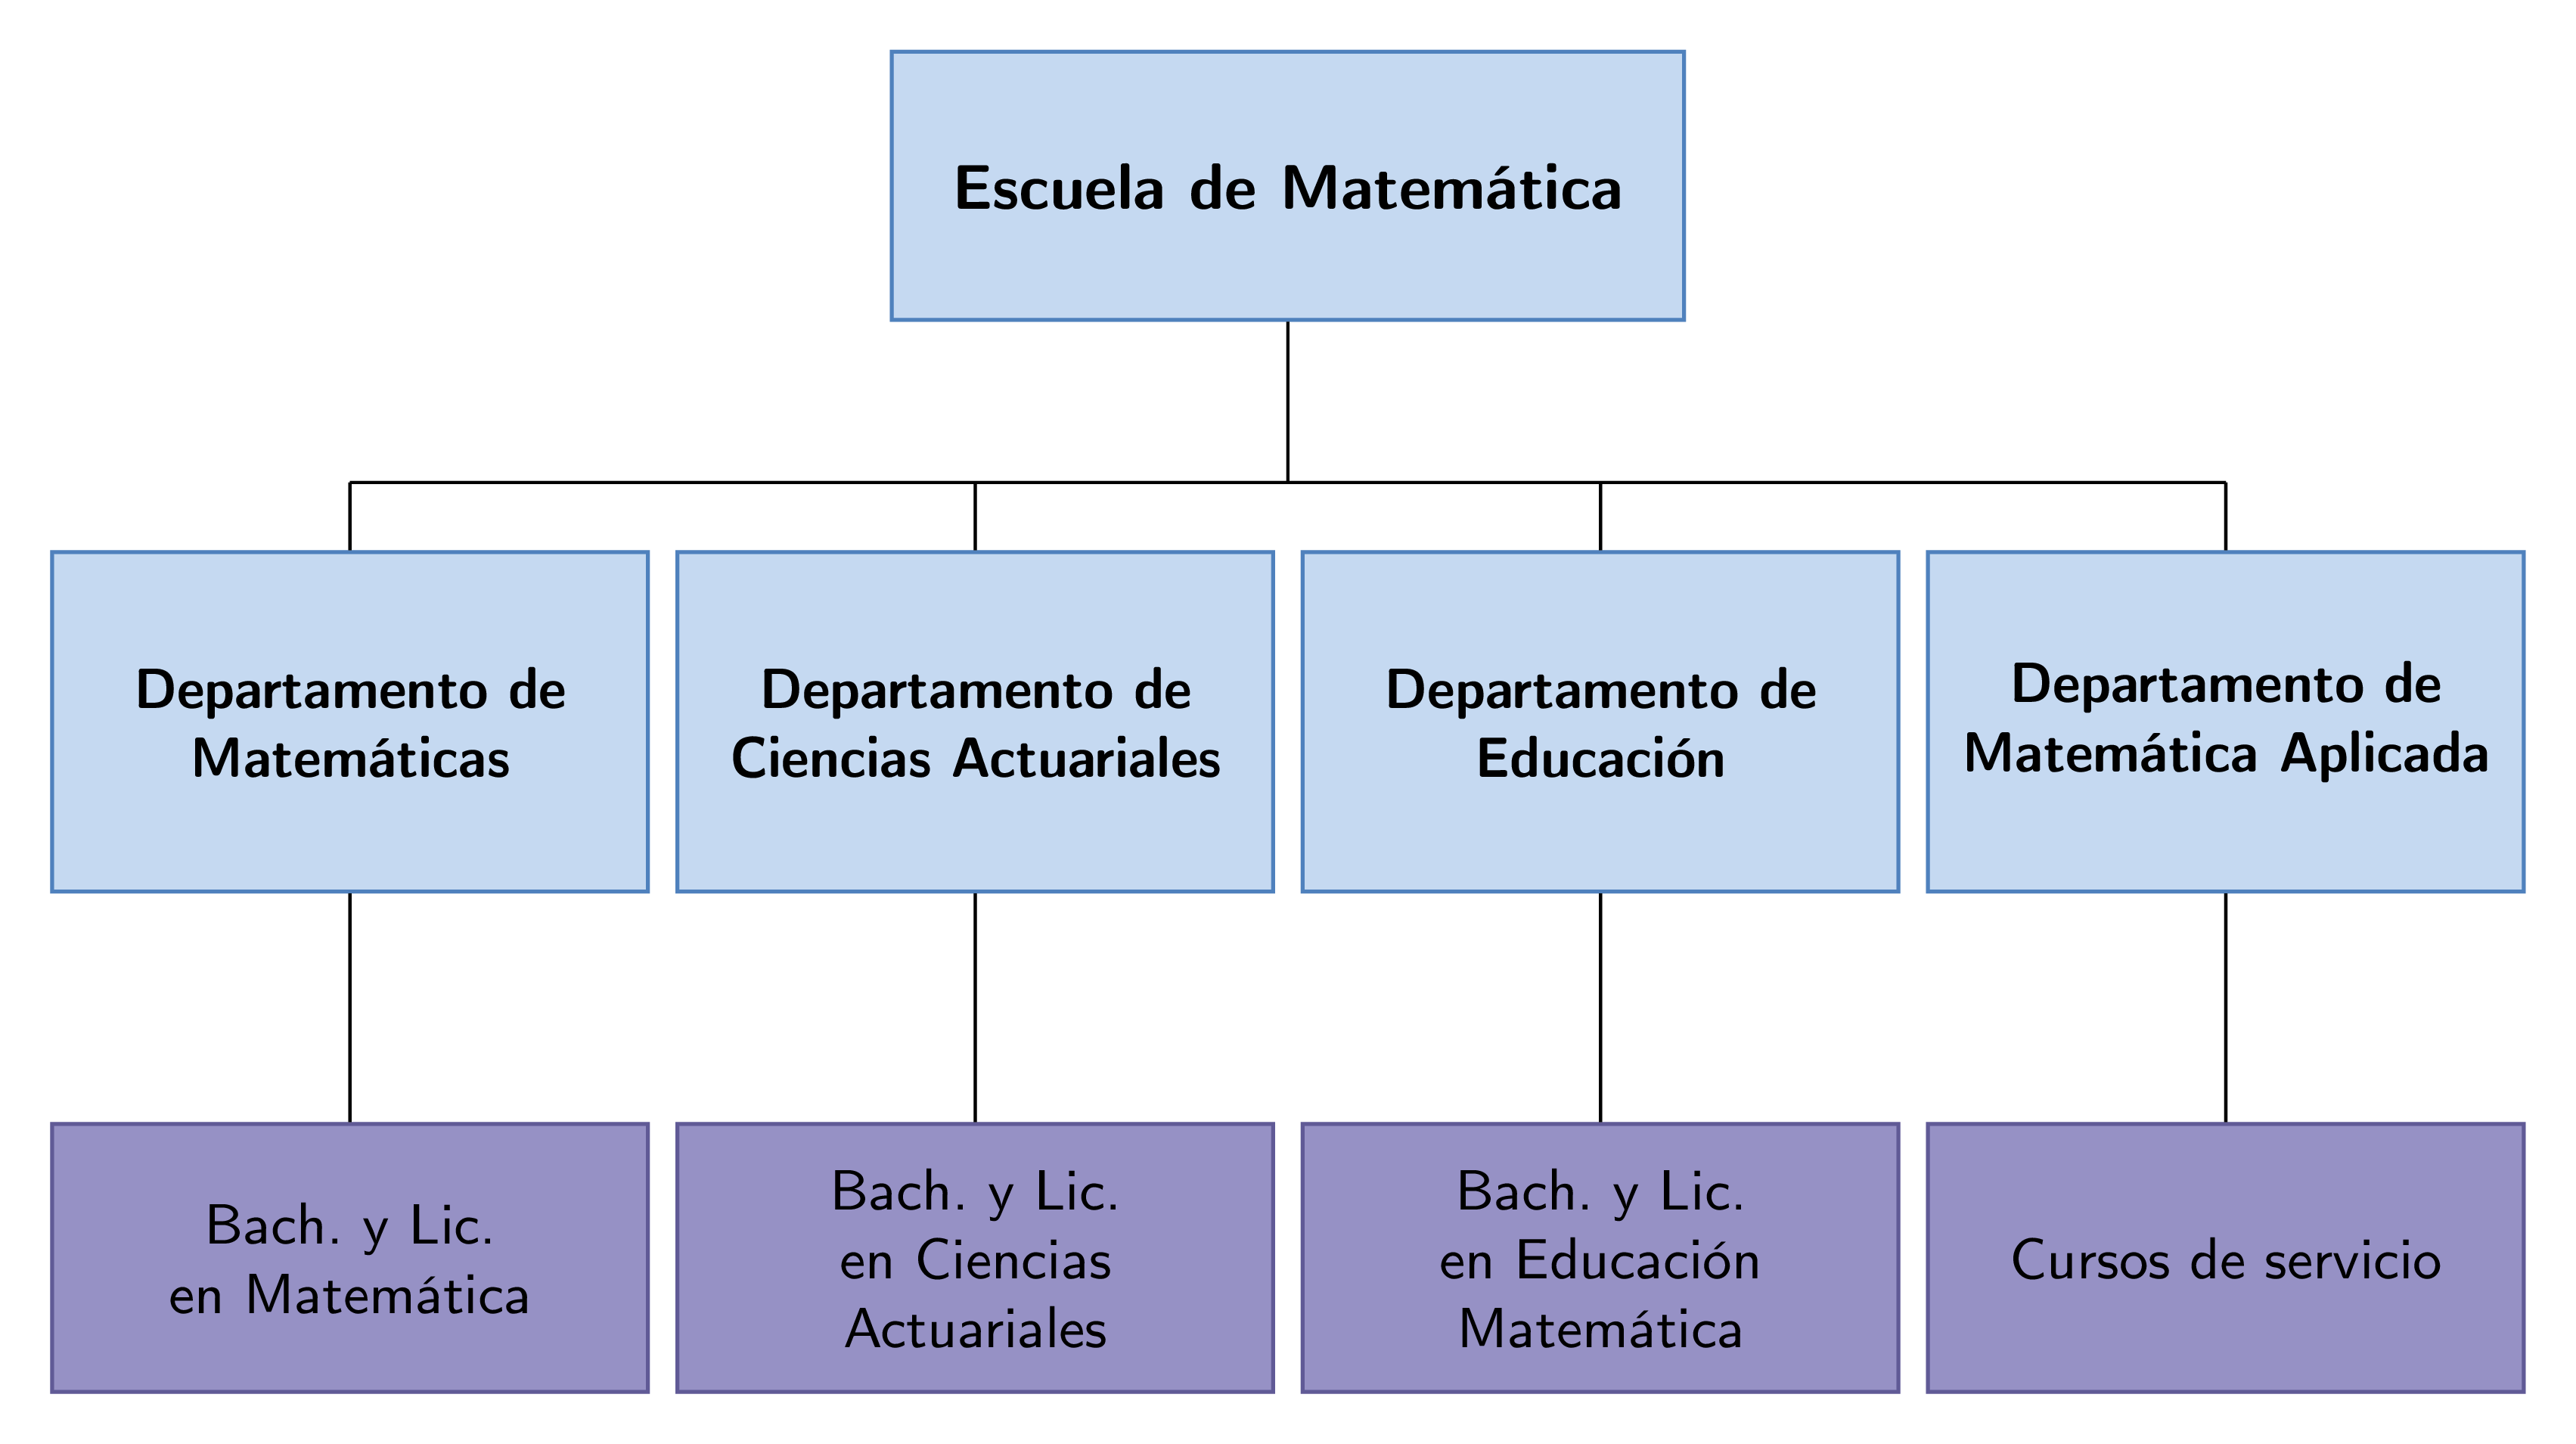
\includegraphics[width=0.5\linewidth]{dptos2.png}
    \caption{División por departamentos vigente en la Escuela de Matemática}
    \label{fig:dpto}
\end{figure}

\subsection{Cuerpo docente}
En la Tabla \ref{tab:docentes} se presenta el personal docente activo que ha impartido cursos en la carrera de Matemática desde el año 2010. Se clasifican por áreas de especialización, que corresponde a la especialización que tiene más cercanía a las áreas curriculares que se definieron con anterioridad. En la última columna de la tabla se especifica si el nombramiento de cada docente es en propiedad (P), becario (B), exbecario (E), o interinazgo (I).

% Please add the following required packages to your document preamble:
% \usepackage{longtable}
% Note: It may be necessary to compile the document several times to get a multi-page table to line up properly
\begin{longtable}[c]{|l|l|c|}
\caption{Lista de docentes en condición activa que han impartido cursos desde el 2010.}
\label{tab:docentes}\\
\hline
\rowcolor[HTML]{00C0F3}
Docente & Especialidad & Nombramiento \\ \hline
%
\endhead
%
Jennifer Acuña Larios & Análisis & P \\ \hline
Luis Acuña Valverde &  & P \\ \hline
Josué Ávila Artavia &  & E \\ \hline
Luis Barboza Chinchilla &  & P \\ \hline
Adrián Barquero Sánchez &  & P \\ \hline
Raúl Bolaños Guerrero &  & P \\ \hline
Ronald Bustamante Medina &  & P \\ \hline
Juan Gabriel Calvo Alpízar &  & P \\ \hline
Santiago Cambronero Villalobos &  & P \\ \hline
José David Campos Fernández &  & P \\ \hline
Daniel Campos Salas &  & P \\ \hline
Santiago Chaves Aguilar &  & E \\ \hline
Pedro Díaz Navarro &  & I \\ \hline
Christian Fonseca Mora &  & P \\ \hline
Álvaro Guevara Villalobos &  & P \\ \hline
Jorge Guier Acosta &  & P \\ \hline
Jonathan Gutiérrez Pavón &  & P \\ \hline
Alberto Hernández Alvarado &  & P \\ \hline
David Jiménez López &  & P \\ \hline
David Krumm Cabezas &  & I \\ \hline
Allan Lacy Mora &  & P \\ \hline
Jennifer Loría Sorio &  & E \\ \hline
Darío Mena Arias &  & P \\ \hline
Pedro Méndez Hernández &  & P \\ \hline
Carlos Montalto Cruz &  & P \\ \hline
Samaria Montenegro Guzmán &  & P \\ \hline
German Mora Sáenz &  & B \\ \hline
Adrián Naranjo Alvarado &  & B \\ \hline
Hugo Peña Gómez &  & I \\ \hline
Alexander Ramírez González &  & P \\ \hline
Oldemar Rodríguez Rojas &  & P \\ \hline
José Rosales Ortega &  & P \\ \hline
Adriana Sánchez Chavarría &  & P \\ \hline
Jesús Sánchez Guevara &  & P \\ \hline
Fabio Sánchez Peña &  & P \\ \hline
Esteban Segura Ugalde &  & P \\ \hline
Filánder Sequeira Chavarría &  & I \\ \hline
Maikol Solís Chacón &  & P \\ \hline
Javier Trejos Zelaya &  & P \\ \hline
William Ugalde Gómez &  & P \\ \hline
Roberto Ulloa Esquivel &  & E \\ \hline
Mario Villalobos Arias &  & P \\ \hline
Mark Villarino Bertran &  & P \\ \hline
Rafael Zamora Calero &  & P \\ \hline
Óscar Zamora Luna &  & E \\ \hline
Ronald Zúñiga Rojas &  & P \\ \hline
\end{longtable}


Con base en la información anterior, se detalla la cantidad de profesores disponibles (no exclusivos) por cada uno de los cursos que componen la malla curricular propuesta en la Tabla \ref{tab:cursos}. Es importante agregar que muchos docentes están simultáneamente disponibles en más de un curso, por lo que esta tabla representa un escenario optimista de la cantidad de recursos disponibles en la Escuela de Matemática para hacerle frente a la oferta académica. Cada curso se espera que sea impartido por docentes con doctorado. En el caso de tener maestría, se permitirá si el  curso es relacionado con el área de trabajo. %Por otro lado, la columna que indica el grado académico mínimo es definido con respecto a la complejidad de los contenidos y a la ubicación del curso en la malla curricular.


\begin{longtable}[c]{|l|p{7cm}|p{3.4cm}|p{2cm}|}
\caption{Número de personal docente por curso del nuevo plan de estudios, según especialidad}
\label{tab:cursos}\\
\hline
\rowcolor[HTML]{00C0F3}
Sigla & Curso & Área de especialidad & Número de docentes \\ \hline
%
\endhead
%
\MA{0151} & \gls{MA0151} & General &  \\ \hline
\MA{0152} & \gls{MA0152} & General &  \\ \hline
\MA{0251} & \gls{MA0251} & General &  \\ \hline
\MA{0252} & \gls{MA0252} & General &  \\ \hline
\MA{0261} & \gls{MA0261} & Álgebra &  \\ \hline
\MA{0341} & \gls{MA0341} & Numérico &  \\ \hline
\MA{0351} & \gls{MA0351} & Análisis &  \\ \hline
\MA{0361} & \gls{MA0361} & Álgebra &  \\ \hline
\MA{0451} & \gls{MA0451} & Análisis &  \\ \hline
\MA{0461} & \gls{MA0461} & Teoría de números &  \\ \hline
\MA{0471} & \gls{MA0471} & Análisis &  \\ \hline
\MA{0472} & \gls{MA0472} & Geometría &  \\ \hline
\MA{0515} & \gls{MA0515} & Análisis &  \\ \hline
\MA{0520} & \gls{MA0520} & Análisis/Estadística &  \\ \hline
\MA{0535} & \gls{MA0535} & Álgebra &  \\ \hline
\MA{0541} & \gls{MA0541} & Numérico &  \\ \hline
\MA{0615} & \gls{MA0615} & Análisis &  \\ \hline
\MA{0625} & \gls{MA0625} & Análisis &  \\ \hline
\MA{0635} & \gls{MA0635} & Álgebra &  \\ \hline
\MA{063X} & \gls{MA063X} & Topología &  \\ \hline
\MA{0702} & \gls{MA0702} & Análisis &  \\ \hline
\MA{0725} & \gls{MA0725} & Análisis &  \\ \hline
\MA{07xx} & \gls{MA07xx} & Geometría &  \\ \hline
\MA{-OPT} & \gls{OPT-Algebra} & Álgebra &  \\ \hline
\MA{-OPT} & \gls{OPT-Analisis} & Análisis &  \\ \hline
\MA{-OPT} & \gls{OPT-Aplicada} & Aplicada &  \\ \hline
\MA{-OPT} & \gls{OPT-Computacion cientifica} & Numérico &  \\ \hline
\MA{-OPT} & \gls{OPT-Discreta} & Discreta &  \\ \hline
\MA{-OPT} & \gls{OPT-Estadistica, Ciencia datos} & Estadística&  \\ \hline
\MA{-OPT} & \gls{OPT-Geometria} & Geometría &  \\ \hline
\MA{-OPT} & \gls{OPT-Logica} & Lógica &  \\ \hline
\MA{-OPT} & \gls{OPT-Topologia} & Topología &  \\ \hline
%\end{tabular}
\end{longtable}


\subsection{Plan de Transición}
Para estudiantes activos que ingresaron en el año 2025 o anteriores, se propone un plan de transición con base en el cohorte que corresponda, bajo el supuesto de que cada estudiante tiene el año correspondiente al cohorte completo al finalizar el año 2025. Los documentos completos se incluyen en el Anexo ??.

\subsubsection{Cohorte C7}
Se estima que este grupo tendrá XX estudiantes, quienes aprobaron MA0150 y MA0250, además de los cursos de generales de primer año. %A este grupo se le debe convalidar MA0251, MA0252 y permitir que MA0261 sea correquisito con los cursos del I26, como excepción por el plan de transición.

\begin{table}[h!]
\centering
\begin{tabular}{|l|l|}
\hline
\rowcolor[HTML]{00C0F3}
Cohorte C7 & Primer año completo del plan anterior \\ \hline
I28 & \begin{tabular}[c]{@{}l@{}}\textbf{Pura y Aplicada:}\\ SR-I Seminario de Realidad Nacional I (2)\\ MA0361 Álgebra Lineal I (4)\\ EG- Curso de Arte (2)\\ MA0351 Cálculo en Varias Variables (4)\\ MA0341 Matemática Computacional (4)\end{tabular} \\ \hline
II28 & \begin{tabular}[c]{@{}l@{}}\textbf{Pura y Aplicada:} igual que el ciclo IV del plan 03\end{tabular} \\ \hline
I29 & \begin{tabular}[c]{@{}l@{}}\textbf{Pura y Aplicada:} igual que el ciclo V del plan 03\end{tabular} \\ \hline
II29 & \begin{tabular}[c]{@{}l@{}}\textbf{Pura y Aplicada:} igual que el ciclo VI del plan 03\end{tabular} \\ \hline
I30 & \begin{tabular}[c]{@{}l@{}}\textbf{Pura y Aplicada:} igual que el ciclo VII del plan 03\end{tabular} \\ \hline
II30 & \begin{tabular}[c]{@{}l@{}}\textbf{Pura y Aplicada:} igual que el ciclo VIII del plan 03\end{tabular} \\ \hline
\end{tabular}
\end{table}

% \begin{table}[h!]
% \centering
% \begin{tabular}{|c|l|}
% \hline
% \rowcolor[HTML]{00C0F3}
% Cohorte C5 & Primer año completo del plan anterior \\ \hline
% I26 & \begin{tabular}[c]{@{}l@{}}MA0261 \gls{MA0261} (3)\\ MA0341 \gls{MA0341} (4)\\ MA0351 \gls{MA0351} (4)\\ Artística (2)\end{tabular} \\ \hline
% II26 & \begin{tabular}[c]{@{}l@{}}MA0361 \gls{MA0361} (4)\\ MA0451 \gls{MA0451} (4)\\ MA0461 \gls{MA0461} (4)\\ MA0471 \gls{MA0471} (4)\\ Seminario de Realidad Nacional I (2)\end{tabular} \\ \hline
% I27 & Igual que Ciclo V - Plan 26 \\ \hline
% II 27 & Igual que Ciclo VI - Plan 26 \\ \hline
% I 28 & Igual que Ciclo VII - Plan 26 \\ \hline
% II 28 & Igual que Ciclo VIII - Plan 26 \\ \hline
% \end{tabular}
% \end{table}

\subsubsection{Cohorte C6}
Se estima que este grupo tendrá XX estudiantes, quienes aprobaron MA0150, MA0250, MA0350, MA0360, MA0370, MA0450 y MA0460. %A este grupo se le debe convalidar MA0252, MA0351, MA0341, y permitir que MA0461 y MA0535 sean correquisitos, como excepción por el plan de transición.

\begin{table}[h!]
\centering
\begin{tabular}{|l|l|}
\hline
\rowcolor[HTML]{00C0F3}
Cohorte C6 & Dos primeros años completos del plan anterior \\ \hline
I28 & \begin{tabular}[c]{@{}l@{}}\textbf{Pura:}\\ MA0561 Álgebra Abstracta I (4)\\ MA0471 Introducción a la Geometría Diferencial (3)\\ MA0515 Ecuaciones Diferenciales Ordinarias (4)\\ Optativa de otra disciplina (3)\\ \textbf{Aplicada:}\\ MA0635 Topología General (4)\\ MA0515 Ecuaciones Diferenciales Ordinarias (4)\\ Optativa específica de matemática (4)\\ Optativa de otra disciplina (4)\end{tabular} \\ \hline
II28 & \begin{tabular}[c]{@{}l@{}}\textbf{Pura:} igual que el ciclo VI del plan 03\\ \textbf{Aplicada:}\\ CA0204 Herramientas de Ciencia de Datos I (4)\\ MA0647 Modelación Matemática (4)\\ CA0721 Probabilidad (4)\\ MA0641 Análisis Numérico I (4)\end{tabular} \\ \hline
I29 & \begin{tabular}[c]{@{}l@{}}\textbf{Pura:} igual que el ciclo VII del plan 03\\ \textbf{Aplicada:}\\ CA0303 Estadística Actuarial I (4)\\ MA0702 Análisis Complejo (4)\\ MA0705 Análisis Real I (4)\\ MA0780 Comunicación en las Ciencias (2)\\ MA0701 Seminario (0)\end{tabular} \\ \hline
II29 & \begin{tabular}[c]{@{}l@{}}\textbf{Pura:} igual que el ciclo VIII del plan 03\\ \textbf{Aplicada:}\\ CA0411 Análisis de Datos I (4)\\ Optativa específica de matemática (4)\\ Optativa específica de matemática (4)\\ MA0781 Pasantía (4)\end{tabular} \\ \hline
\end{tabular}
\end{table}

% \begin{table}[h!]
% \centering
% \begin{tabular}{|l|l|}
% \hline
% \rowcolor[HTML]{00C0F3}
% Cohorte C4 & Segundo año completo del plan anterior) \\ \hline
% I26 & \begin{tabular}[c]{@{}l@{}} {MA0561} (4), MA0515 (4), MA0471 (3), optativa otra disciplina\\ Aplicada: CA0721, CA0203, MA0515, optativa \\
% **MA0461 \gls{MA0461} (4)\\ MA0520 \gls{MA0520} (4)\\ MA0535 \gls{MA0535} (4)\\ MA0541 \gls{MA0541} (4)\\ Seminario de Realidad Nacional II (2)\end{tabular} \\ \hline
% II26 & Igual que Ciclo VI - Plan 26\\ Aplicada: \\ \hline
% I27 & Igual que Ciclo VII - Plan 26\\ Aplicada: \\ \hline
% II 27 & Igual que Ciclo VIII - Plan 26\\ Aplicada: \\ \hline
% \end{tabular}
% \end{table}

\subsubsection{Cohorte C5}
Quienes tengan tres años completos del plan 02, deben finalizar dicho plan. Para ello deben cursar MA0702, MA0704, MA0870, una optativa de otra disciplina y tres optativas de Matemática. Posteriormente, podrán continuar en la licenciatura del plan 03.

\subsubsection{Excepciones}
Cada estudiante que no haya cumplido sus ciclos de estudio de acuerdo con el plan de estudios anterior, no contemplados en los incisos anteriores, o aquellos de planes previos, deberá de utilizar la tabla de convalidaciones para trasladarse hacia la malla del nuevo plan de estudios, y deberá cursar los cursos no convalidables hasta cumplir con todos los requisitos del plan 2028. 

\subsubsection{Convalidaciones}

Se plantea considerar convalidaciones para casos particulares que no cumplen con un cohorte específico; ver Tabla \ref{tab:conv}. De esta forma, se deberán trasladar al Plan 03 que inicia en el 2028, realizando las convalidaciones que correspondan, y deberán cursar aquellos cursos no convalidables hasta cumplir con todos los requisitos del plan 2028.

\begin{table}[h!]
\centering
\caption{Convalidaciones para la transición de plan de estudios}
\label{tab:conv}
\begin{tabular}{|p{7.25cm}|p{7.25cm}|}
\rowcolor[HTML]{00C0F3}
\hline
Sigla y curso aprobado & Sigla y curso por convalidar \\ \hline
MA0150 Principios de Matemática & MA0252 Introducción a las Demostraciones \\ \hline
MA0250 Cálculo en una Variable I & MA0251 Cálculo en una Variable \\ \hline
MA0350 Cálculo en una Variable II & MA0451 Principios de Análisis I \\ \hline
MA0360 Álgebra Lineal I & MA0361 Álgebra Lineal I \\ \hline
MA0370 Principios de Geometría & MA0496 Teoría de Números u Optativa Específica de Matemática \\ \hline
MA0450 Cálculo en Varias Variables & MA0551 Principios de Análisis II \\ \hline
MA0455 Ecuaciones Diferenciales Ordinarias & MA0515 Ecuaciones Diferenciales Ordinarias \\ \hline
MA0460 Álgebra Lineal II & MA0461 Álgebra Lineal II \\ \hline
MA0505 Análisis I & MA0705 Análisis Real I \\ \hline
MA0561 Grupos y Anillos & MA0561 Álgebra Abstracta I \\ \hline
MA0605 Análisis II & MA0725 Análisis Real II \\ \hline
MA0660 Teoría de Galois & MA0661 Álgebra Abstracta II \\ \hline
MA0702 Variable Compleja I & MA0702 Análisis Complejo \\ \hline
MA0704 Topología General I & MA0635 Topología General \\ \hline
MA0870 Geometría Diferencial & MA0471 Introducción a la Geometría Diferencial \\ \hline
OPT- Bloque de Optativos Específicos de Matemáticas & Optativa Específica de Matemática \\ \hline
Cursos de Licenciatura & Optativa Específica de Matemática \\ \hline
\end{tabular}
\end{table}

\subsection{Proyección de carga académica para el plan de transición}

Según el plan descrito en la sección anterior, se presenta la proyección de carga académica necesaria para suplir la demanda de los años de transición (2028, 2029, 2030). Esto bajo el supuesto de recibir el máximo de 26 estudiantes por año más doce estudiantes por traslado, ofertando dos grupos? por curso en primer año.

\begin{longtable}[c]{|p{0.7cm}|p{1.6cm}|p{6.4cm}|p{1.5cm}|p{1.2cm}|p{1.4cm}|}
\caption{Proyección de carga académica para el plan de transición, año 2028}
\label{tab:carga2028}\\
\hline
\rowcolor[HTML]{00C0F3}
Ciclo & Cohorte & Curso & Créditos & Grupos & Jornada \\ \hline
\endhead
%
I & C8P C8A & MA0151 Fundamentos de Álgebra, Trigonometría y Geometría Analítica & 3 & \textbf{2} & 0.375 \\ \hline
I & C8P C8A & MA0152 Matemática Exploratoria & 3 & \textbf{2} & 0.375 \\ \hline
I & C7P C7A & MA0341 Matemática Computacional & 4 & 1 & 0.375 \\ \hline
I & C7P C7A & MA0351 Cálculo en Varias Variables & 4 & 1 & 0.375 \\ \hline
I & C7P C7A & MA0361 Álgebra Lineal I & 4 & 1 & 0.375 \\ \hline
I & C6P & MA0471 Introducción a la Geometría Diferencial & 3 & 1 & 0.375 \\ \hline
I & C6P C6A & MA0515 Ecuaciones Diferenciales Ordinarias & 4 & 1 & 0.375 \\ \hline
I & C6P & MA0561 Álgebra Abstracta I & 4 & 1 & 0.375 \\ \hline
I & C6A & MA0635 Topología General & 4 & 1 & 0.375 \\ \hline
I & C5 & MA0702 Variable Compleja I & 5 & 1 & 0.375 \\ \hline
I & C5 & MA0704 Topología General I & 5 & 1 & 0.000 \\ \hline
I & C5 C6A& OPT- Bloque de Optativos Específicos de Matemáticas & 5 & 1 & 0.375 \\ \hline
%I & C6A & OPT- Optativa Específica de Matemática & 4 & 1 & 0.375 \\ \hline
 &  &  & Subtotal I Ciclo & 14 & 3.575 \\ \hline
II & C6A C7A & CA0204 Herramientas de Ciencia de Datos I & 4 & 1 & 0.375 \\ \hline
II & C6A C7A & CA0721 Probabilidad & 4 & 1 & 0.375 \\ \hline
II & C8P C8A & LM3039 Inglés para Estadística I & 3 & 1 & 0.250 \\ \hline
II & C8P C8A & MA0251 Cálculo en una Variable & 3 & 1 & 0.375 \\ \hline
II & C8P C8A & MA0252 Introducción a las Demostraciones & 4 & 1 & 0.375 \\ \hline
II & C7P C7A & MA0451 Principios de Análisis I & 4 & 1 & 0.375 \\ \hline
II & C7P C7A & MA0461 Álgebra Lineal II & 4 & 1 & 0.375 \\ \hline
II & C7P & MA0471 Introducción a la Geometría Diferencial & 3 & 1 & 0.375 \\ \hline
II & C7P & MA0496 Teoría de Números & 3 & 1 & 0.375 \\ \hline
II & C6P & MA0635 Topología General & 4 & 1 & 0.375 \\ \hline
II & C6P C6A & MA0641 Análisis Numérico I & 4 & 1 & 0.375 \\ \hline
II & C6A & MA0647 Modelación Matemática & 4 & 1 & 0.375 \\ \hline
II & C6P & MA0661 Álgebra Abstracta II & 4 & 1 & 0.375 \\ \hline
II & C5 & MA0870 Geometría Diferencial & 5 & 1 & 0.375 \\ \hline
II & C5 & OPT- Bloque de Optativos Específicos de Matemáticas & 5 & 1 & 0.375 \\ \hline
II & C5 & OPT- Bloque de Optativos Específicos de Matemáticas & 5 & 1 & 0.375 \\ \hline
 &  &  & Subtotal II Ciclo & 16 & 5.875 \\ \hline
 &  &  & Total del año & 29 & 9.450 \\ \hline
\end{longtable}

\begin{longtable}[c]{|p{0.8cm}|p{1.8cm}|p{6.8cm}|p{1.5cm}|p{1.3cm}|p{1.5cm}|}
\caption{Proyección de carga académica para el plan de transición, año 2029}
\label{tab:carga2029}\\
\hline
\rowcolor[HTML]{00C0F3}
Ciclo & Cohorte & Curso & Créditos & Grupos & Jornada \\ \hline
\endhead
%
I & C6A C7A & CA0303 Estadística Actuarial I & 4 & 1 & 0.375 \\ \hline
I & C8P C8A & LM3040 Inglés para Estadística II & 3 & 1 & 0.250 \\ \hline
I & C9P C9A & MA0151 Fundamentos de Álgebra, Trigonometría y Geometría Analítica & 3 & 1 & 0.375 \\ \hline
I & C9P C9A & MA0152 Matemática Exploratoria & 3 & 1 & 0.375 \\ \hline
I & C8P C8A & MA0341 Matemática Computacional & 4 & 1 & 0.375 \\ \hline
I & C8P C8A & MA0351 Cálculo en Varias Variables & 4 & 1 & 0.375 \\ \hline
I & C8P C8A & MA0361 Álgebra Lineal I & 4 & 1 & 0.375 \\ \hline
I & C7P C7A & MA0515 Ecuaciones Diferenciales Ordinarias & 4 & 1 & 0.375 \\ \hline
I & C7P C7A & MA0551 Principios de Análisis II & 4 & 1 & 0.375 \\ \hline
I & C7P & MA0561 Álgebra Abstracta I & 4 & 1 & 0.375 \\ \hline
I & C6P C6A & MA0701 Seminario & 0 & 1 & 0.000 \\ \hline
I & C6P C6A & MA0702 Análisis Complejo & 4 & 1 & 0.375 \\ \hline
I & C6P C6A & MA0705 Análisis Real I & 4 & 1 & 0.375 \\ \hline
I & C6P C6A & MA0780 Comunicación en las Ciencias & 2 & 1 & 0.375 \\ \hline
I & C6P & OPT- Optativa Específica de Matemática & 4 & 1 & 0.375 \\ \hline
 &  &  & Subtotal I Ciclo & 15 & 5.4375 \\ \hline
II & C8A & CA0204 Herramientas de Ciencia de Datos I & 4 & 1 & 0.375 \\ \hline
II & C6A & CA0411 Análisis de Datos I & 4 & 1 & 0.375 \\ \hline
II & C8A & CA0721 Probabilidad & 4 & 1 & 0.375 \\ \hline
II & C9P C9A & LM3039 Inglés para Estadística I & 3 & 1 & 0.1875 \\ \hline
II & C9P C9A & MA0251 Cálculo en una Variable & 3 & 1 & 0.375 \\ \hline
II & C9P C9A & MA0252 Introducción a las Demostraciones & 4 & 1 & 0.375 \\ \hline
II & C8P C8A & MA0451 Principios de Análisis I & 4 & 1 & 0.375 \\ \hline
II & C8P C8A & MA0461 Álgebra Lineal II & 4 & 1 & 0.375 \\ \hline
II & C8P & MA0471 Introducción a la Geometría Diferencial & 3 & 1 & 0.375 \\ \hline
II & C8P & MA0496 Teoría de Números & 3 & 1 & 0.375 \\ \hline
II & C7P C7A & MA0635 Topología General & 4 & 1 & 0.375 \\ \hline
II & C7P C7A & MA0641 Análisis Numérico I & 4 & 1 & 0.375 \\ \hline
II & C7A & MA0647 Modelación Matemática & 4 & 1 & 0.375 \\ \hline
II & C7P & MA0661 Álgebra Abstracta II & 4 & 1 & 0.375 \\ \hline
II & C6P C6A & MA0781 Pasantía & 4 & 1 & 0.000 \\ \hline
II & C6P C6A & OPT- Optativa Específica de Matemática & 4 & 1 & 0.375 \\ \hline
II & C6P C6A & OPT- Optativa Específica de Matemática & 4 & 1 & 0.375 \\ \hline
II & C6P & OPT- Optativa Específica de Matemática & 4 & 1 & 0.375 \\ \hline
 &  &  & Subtotal II Ciclo & 18 & x.5625 \\ \hline
 &  &  & Total del año & 33 & xx \\ \hline
\end{longtable}

% anchos de columna: Ciclo | Cohorte | Curso | Créditos | Grupos | Jornada
\begin{longtable}[c]{|p{0.8cm}|p{1.8cm}|p{6.8cm}|p{1.5cm}|p{1.3cm}|p{1.5cm}|}
\caption{Proyección de carga académica para el plan de transición, año 2030}
\label{tab:carga2030}\\
\hline
\rowcolor[HTML]{00C0F3}
Ciclo & Cohorte & Curso & Créditos & Grupos & Jornada \\ \hline
\endhead
%
I & C8A & CA0303 Estadística Actuarial I & 4 & 1 & 0.375 \\ \hline
I & C7A & CA0411 Análisis de Datos I & 4 & 1 & 0.375 \\ \hline
I & C9P C9A & LM3040 Inglés para Estadística II & 3 & 1 & 0.1875 \\ \hline
I & C10P C10A & MA0151 Fundamentos de Álgebra, Trigonometría y Geometría Analítica & 3 & 1 & 0.375 \\ \hline
I & C10P C10A & MA0152 Matemática Exploratoria & 3 & 1 & 0.375 \\ \hline
I & C9P C9A & MA0341 Matemática Computacional & 4 & 1 & 0.375 \\ \hline
I & C9P C9A & MA0351 Cálculo en Varias Variables & 4 & 1 & 0.375 \\ \hline
I & C9P C9A & MA0361 Álgebra Lineal I & 4 & 1 & 0.375 \\ \hline
I & C8P C8A & MA0515 Ecuaciones Diferenciales Ordinarias & 4 & 1 & 0.375 \\ \hline
I & C8P C8A & MA0551 Principios de Análisis II & 4 & 1 & 0.375 \\ \hline
I & C8P & MA0561 Álgebra Abstracta I & 4 & 1 & 0.375 \\ \hline
I & C7P C7A & MA0701 Seminario & 0 & 1 & 0.375 \\ \hline
I & C7P C7A & MA0702 Análisis Complejo & 4 & 1 & 0.375 \\ \hline
I & C7P C7A & MA0705 Análisis Real I & 4 & 1 & 0.375 \\ \hline
I & C7P C7A & MA0780 Comunicación en las Ciencias & 2 & 1 & 0.375 \\ \hline
I & C7P & OPT- Optativa Específica de Matemática & 4 & 1 & 0.375 \\ \hline
 &  &  & Subtotal I Ciclo & 16 & 5.8125 \\ \hline
II & C9A & CA0204 Herramientas de Ciencia de Datos I & 4 & 1 & 0.375 \\ \hline
II & C9A & CA0721 Probabilidad & 4 & 1 & 0.375 \\ \hline
II & C10P C10A & LM3039 Inglés para Estadística I & 3 & 1 & 0.1875 \\ \hline
II & C10P C10A & MA0251 Cálculo en una Variable & 3 & 1 & 0.375 \\ \hline
II & C10P C10A & MA0252 Introducción a las Demostraciones & 4 & 1 & 0.375 \\ \hline
II & C9P C9A & MA0451 Principios de Análisis I & 4 & 1 & 0.375 \\ \hline
II & C9P C9A & MA0461 Álgebra Lineal II & 4 & 1 & 0.375 \\ \hline
II & C9P & MA0471 Introducción a la Geometría Diferencial & 3 & 1 & 0.375 \\ \hline
II & C9P & MA0496 Teoría de Números & 3 & 1 & 0.375 \\ \hline
II & C8P C8A & MA0635 Topología General & 4 & 1 & 0.375 \\ \hline
II & C8P C8A & MA0641 Análisis Numérico I & 4 & 1 & 0.375 \\ \hline
II & C8A & MA0647 Modelación Matemática & 4 & 1 & 0.375 \\ \hline
II & C8P & MA0661 Álgebra Abstracta II & 4 & 1 & 0.375 \\ \hline
II & C7P C7A & MA0781 Pasantía & 4 & 1 & 0.375 \\ \hline
II & C7P C7A & OPT- Optativa Específica de Matemática & 4 & 1 & 0.375 \\ \hline
II & C7P C7A & OPT- Optativa Específica de Matemática & 4 & 1 & 0.375 \\ \hline
II & C7P C7A & OPT- Optativa Específica de Matemática & 4 & 1 & 0.375 \\ \hline
 &  &  & Subtotal II Ciclo & 17 & 6.1875 \\ \hline
 &  &  & Total del año & 33 & 12 \\ \hline
\end{longtable}

% anchos de columna: Ciclo | Cohorte | Curso | Créditos | Grupos | Jornada
\begin{longtable}[c]{|p{0.8cm}|p{1.8cm}|p{6.8cm}|p{1.5cm}|p{1.3cm}|p{1.5cm}|}
\caption{Proyección de carga académica para el plan de transición, año 2031}
\label{tab:carga2031}\\
\hline
\rowcolor[HTML]{00C0F3}
Ciclo & Cohorte & Curso & Créditos & Grupos & Jornada \\ \hline
\endhead
%
I & C9A & CA0303 Estadística Actuarial I & 4 & 1 & 0.375 \\ \hline
I & C8A & CA0411 Análisis de Datos I & 4 & 1 & 0.375 \\ \hline
I & C10P C10A & LM3040 Inglés para Estadística II & 3 & 1 & 0.1875 \\ \hline
I & C11P C11A & MA0151 Fundamentos de Álgebra, Trigonometría y Geometría Analítica & 3 & 1 & 0.375 \\ \hline
I & C11P C11A & MA0152 Matemática Exploratoria & 3 & 1 & 0.375 \\ \hline
I & C10P C10A & MA0341 Matemática Computacional & 4 & 1 & 0.375 \\ \hline
I & C10P C10A & MA0351 Cálculo en Varias Variables & 4 & 1 & 0.375 \\ \hline
I & C10P C10A & MA0361 Álgebra Lineal I & 4 & 1 & 0.375 \\ \hline
I & C9P C9A & MA0515 Ecuaciones Diferenciales Ordinarias & 4 & 1 & 0.375 \\ \hline
I & C9P C9A & MA0551 Principios de Análisis II & 4 & 1 & 0.375 \\ \hline
I & C9P & MA0561 Álgebra Abstracta I & 4 & 1 & 0.375 \\ \hline
I & C8P C8A & MA0701 Seminario & 0 & 1 & 0.375 \\ \hline
I & C8P C8A & MA0702 Análisis Complejo & 4 & 1 & 0.375 \\ \hline
I & C8P C8A & MA0705 Análisis Real I & 4 & 1 & 0.375 \\ \hline
I & C8P C8A & MA0780 Comunicación en las Ciencias & 2 & 1 & 0.375 \\ \hline
I & C8P & OPT- Optativa Específica de Matemática & 4 & 1 & 0.375 \\ \hline
 &  &  & Subtotal I Ciclo & 16 & 5.8125 \\ \hline
II & C10A & CA0204 Herramientas de Ciencia de Datos I & 4 & 1 & 0.375 \\ \hline
II & C10A & CA0721 Probabilidad & 4 & 1 & 0.375 \\ \hline
II & C11P C11A & LM3039 Inglés para Estadística I & 3 & 1 & 0.1875 \\ \hline
II & C11P C11A & MA0251 Cálculo en una Variable & 3 & 1 & 0.375 \\ \hline
II & C11P C11A & MA0252 Introducción a las Demostraciones & 4 & 1 & 0.375 \\ \hline
II & C10P C10A & MA0451 Principios de Análisis I & 4 & 1 & 0.375 \\ \hline
II & C10P C10A & MA0461 Álgebra Lineal II & 4 & 1 & 0.375 \\ \hline
II & C10P & MA0471 Introducción a la Geometría Diferencial & 3 & 1 & 0.375 \\ \hline
II & C10P & MA0496 Teoría de Números & 3 & 1 & 0.375 \\ \hline
II & C9P C9A & MA0635 Topología General & 4 & 1 & 0.375 \\ \hline
II & C9P C9A & MA0641 Análisis Numérico I & 4 & 1 & 0.375 \\ \hline
II & C9A & MA0647 Modelación Matemática & 4 & 1 & 0.375 \\ \hline
II & C9P & MA0661 Álgebra Abstracta II & 4 & 1 & 0.375 \\ \hline
II & C8P C8A & MA0781 Pasantía & 4 & 1 & 0.375 \\ \hline
II & C8P C8A & OPT- Optativa Específica de Matemática & 4 & 1 & 0.375 \\ \hline
II & C8P C8A & OPT- Optativa Específica de Matemática & 4 & 1 & 0.375 \\ \hline
II & C8P C8A & OPT- Optativa Específica de Matemática & 4 & 1 & 0.375 \\ \hline
 &  &  & Subtotal II Ciclo & 17 & 6.1875 \\ \hline
 &  &  & Total del año & 33 & 12 \\ \hline
\end{longtable}

% anchos de columna: Año | Grupos I | Jornada I | Grupos II | Jornada II | Total grupos | Jornada total
\begin{longtable}[c]{|p{1.2cm}|p{2cm}|p{2.1cm}|p{2cm}|p{2.1cm}|p{1.9cm}|p{2cm}|}
\caption{Resumen de la proyección de carga académica, 2028--2031 [NO ESTA ACTUALIZADA]}
\label{tab:cargaresumen}\\
\hline
\rowcolor[HTML]{00C0F3}
Año & Grupos I Ciclo & Jornada I Ciclo & Grupos II Ciclo & Jornada II Ciclo & Total grupos & Jornada total \\ \hline
\endhead
%
2028 & 13 & 4.875 & 16 & 5.8125 & 29 & 10.6875 \\ \hline
2029 & 15 & 5.4375 & 18 & 6.5625 & 33 & 12 \\ \hline
2030 & 16 & 5.8125 & 17 & 6.1875 & 33 & 12 \\ \hline
2031 & 16 & 5.8125 & 17 & 6.1875 & 33 & 12 \\ \hline
%Total &  &  &  &  & 128 & 46.6875 \\ \hline
\end{longtable}


\section{Seguimiento y Evaluación}

En esta sección se plantea la estrategia de evaluación de la carrera y el plan de desarrollo docente que la Escuela de Matemática podría implementar para capacitar al cuerpo docente ante las nuevas exigencias académicas de la malla propuesta.

\subsection{Momentos y estrategias de evaluación de la carrera}

La puesta en marcha de esta propuesta estará a cargo de la persona directora del Departamento de Matemática, en conjunto con la comisión que elaboró esta propuesta, quienes supervisarán la implementación completa del proceso de transición y la asignación y ejecución de carga presupuestaria tal y como se detalla en la Sección 5.1. Asimismo, será el Departamento de Matemática el encargado de ejecutar las estrategias de desarrollo docente que se explican en la siguiente sección, preferiblemente a través de la conformación de una comisión con ese objetivo en particular. 
Por otro lado, se recomienda que el Departamento nombre una comisión encargada de la evaluación de la malla curricular propuesta para que tenga listo un diagnóstico del perfil de salida y de la malla vigente a lo sumo cinco años después de que el plan se haya incorporado de manera completa en la población estudiantil. Se recomienda que los mismos miembros que conformaron la elaboración de este documento participen en esa comisión de evaluación.

\subsection{Desarrollo docente}

\subsection{Presupuesto}

